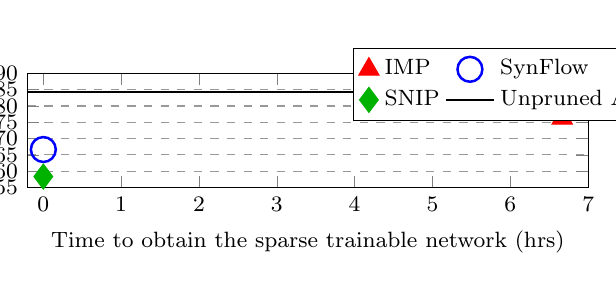
\begin{tikzpicture}[trim axis left,trim axis right,scale=1]
  \begin{axis}[
    width=8.7cm,
    height=0.25\textwidth,
    xlabel={Time to obtain the sparse trainable network (hrs)},
    ylabel={Test accuracy (\%)},
    xmin=-0.2, xmax=7,
    ymin=55, ymax=90,
    xtick={0,1,2,3,4,5,6,7},
    ytick={55,60,65,70,75,80,85,90},
    ymajorgrids=true,
    grid style={dashed,black!40},
    tick label style={font=\footnotesize},
    label style={font=\footnotesize},
    legend style={
      font=\footnotesize,
      cells={anchor=west},
      legend columns=2,
      draw=black, fill=white, inner sep=2pt,
      at={(0.58,0.58)}, anchor=south west
    },
    legend cell align=left,
    mark options={scale=1.5},
  ]

    % IMP
    \addplot[
      only marks,
      mark=triangle*,
      color=red,
      mark size=2.8pt
    ] coordinates {(24000/3600, 76.24)};
    \addlegendentry{IMP}

    % SynFlow
    \addplot[
      only marks,
      mark=o,
      draw=blue, fill=white,
      line width=0.9pt,
      mark size=3pt
    ] coordinates {(4.2/3600, 66.64)};
    \addlegendentry{SynFlow}

    % SNIP
    \addplot[
      only marks,
      mark=diamond*,
      color=green!70!black,
      mark size=3pt
    ] coordinates {(3.13/3600, 58.35)};
    \addlegendentry{SNIP}

    % Unpruned accuracy (horizontal reference line)
    \addplot[mark=none, black, thick]
      coordinates {(-0.2,84.2) (7,84.2)};
    \addlegendentry{Unpruned Accuracy}

  \end{axis}
\end{tikzpicture}